\subsection{Simplified motor model}
The motor is a \textit{Motenergy ME1117 PMAC Motor}. Its parameters can be seen in table \ref{Motor_parameters_list}.

\begin{table} [H]
    \centering
    \begin{tabular}{|c|c|} \cline{1-2}
        \textbf{Parameters} & \textbf{Number} \\ \cline{1-2}
        \textbf{Pole pair} & $4\ pairs\ (8\ poles)$ \\ \cline{1-2}
        \textbf{Phase to Phase R} & $0.013\ohm$ \\ \cline{1-2}
        \textbf{Maximum rotational speed} & $5000$ \textit{RPM} \\ \cline{1-2}
        \textbf{Voltage rating} & $0-76$ \textit{Volts} \\ \cline{1-2}
        \textbf{Torque constant} & $0.13$ \textit{Nm/A} \\ \cline{1-2}
        \textbf{Inductance Phase to Phase} & $0.1$ \textit{mH} \\ \cline{1-2}
        \textbf{Armature Inertia} & $52\ kg/cm^2$ \\ \cline{1-2}
        \textbf{Continuous current} & $100\ A$ \\ \cline{1-2}
        \textbf{Peak Current for 1 min} & $300\ A$ \\ \cline{1-2}  
    \end{tabular} \\
    \caption{Motor parameters as seen in \cite{Motor_Parameters}}
    \label{Motor_parameters_list}
\end{table} \\

All of these specifications are what makes up the motor, and will be written into the model motor. It will also be used in order to calculate framework of the controller. Before diving in to the specifics of how and why, certain methods is used. A quick overview of the base model, will help visualize how the final model was made.\\

\begin{figure} [H]
    \centering
    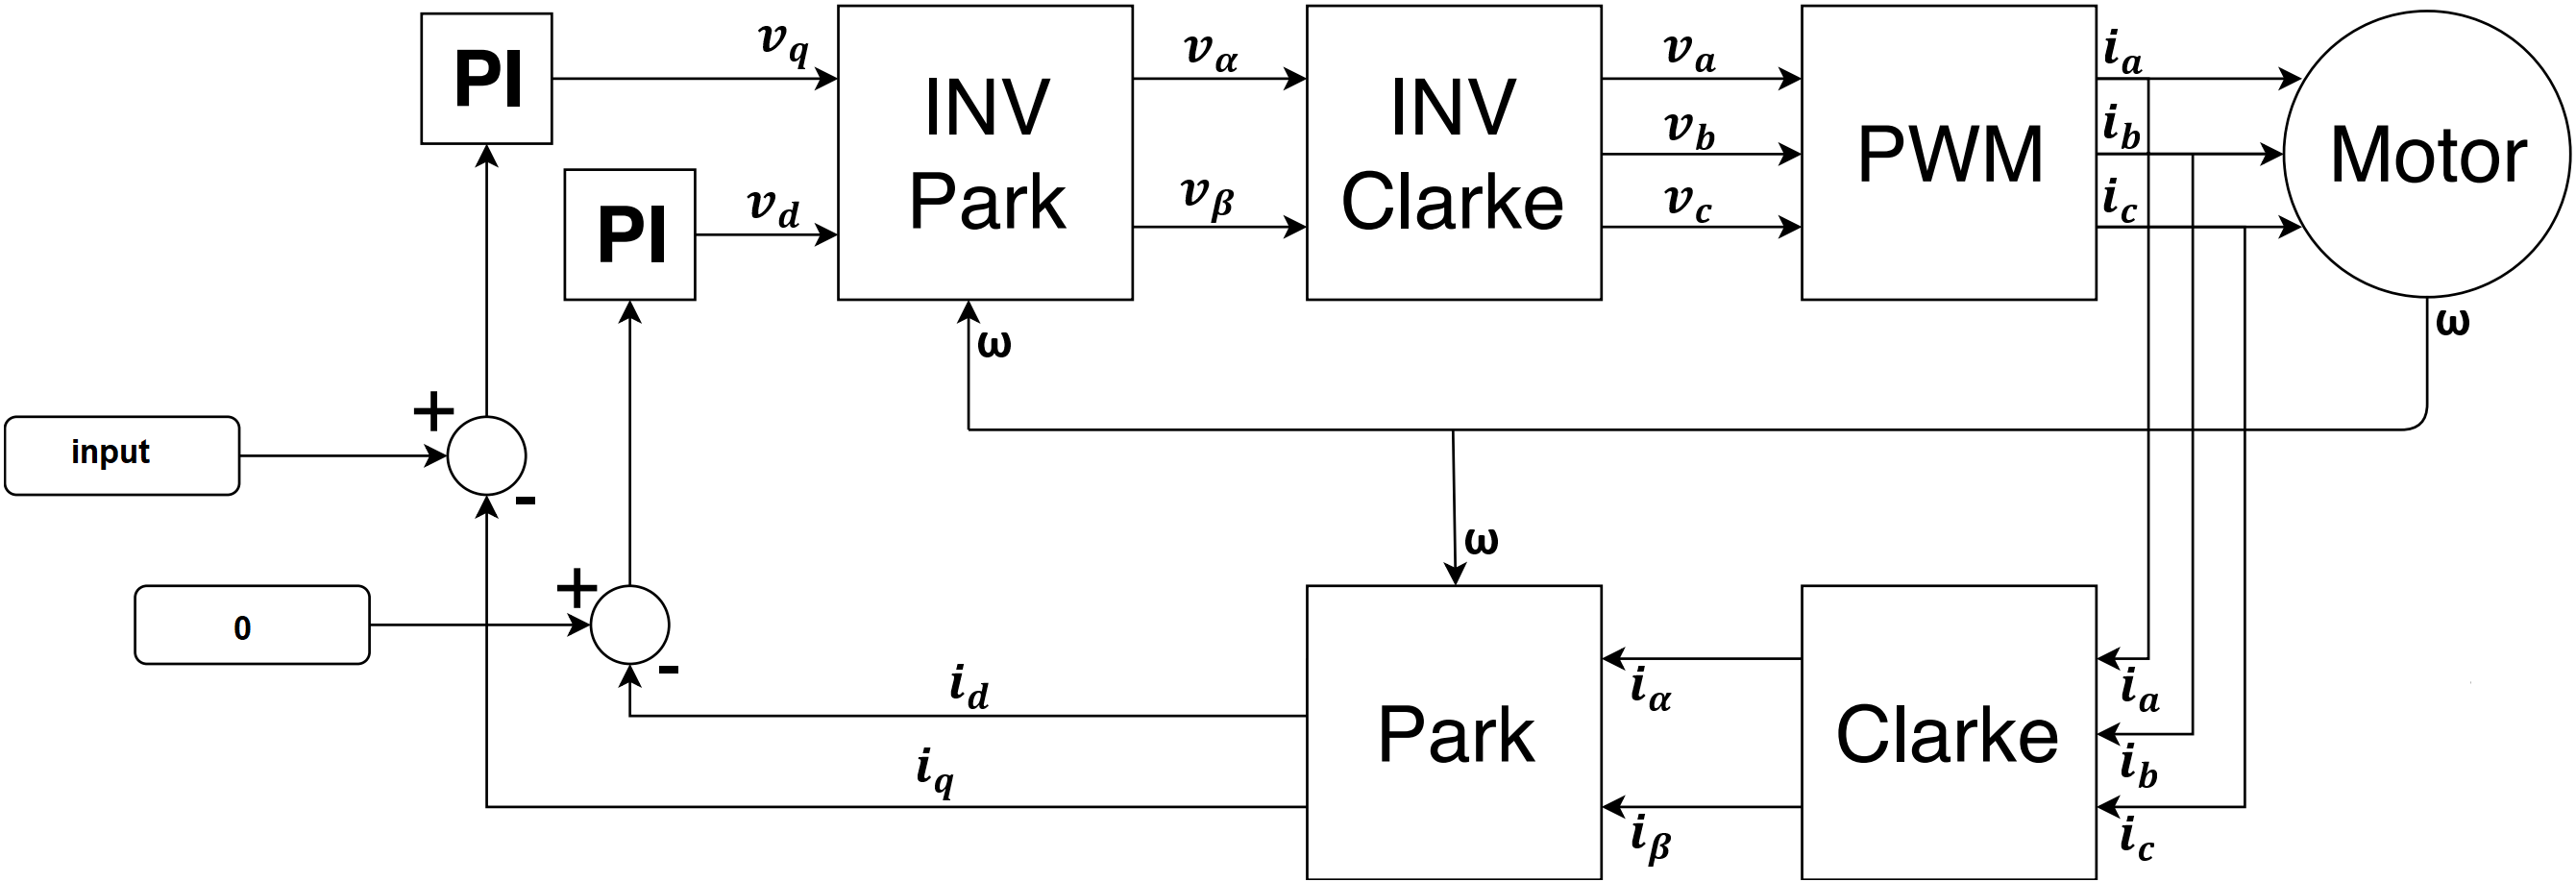
\includegraphics[scale=0.42]{pictures/control/udklip.PNG}
    \caption{Motor model used for the control as an overview.}
    \label{fig:Motor_model}
\end{figure} \\

As seen in \ref{fig:Motor_model} the model consist of two inputs, two PI controllers, and inverse Park and Clarke transformations, a motor with the data from \ref{Motor_parameters_list} and negative feedback transformed back with normal Park, Clarke transformation.\\

The general idea behind model is having the input, being the wanted speed of the motor as a current, in go karts case it would be the torque pedal. The $0$ input is $0$ because of field oriented control, more on that in next section. The signal is then being tuned with the negative feedback and the controllers. Having the signal transformed is an important step, since a 3-phase motors needs 3 signals. The PWM box adjust the actual speed of the motor. The feedback comes from the 3 phases and the speed, that all help minimize errors in the signal. \\

\subsubsection{Field oriented control}
There are in motor control, a couple of common techniques used. It could be scalar based or vector based, each having their usages. \\

\begin{figure} [H]
    \centering
    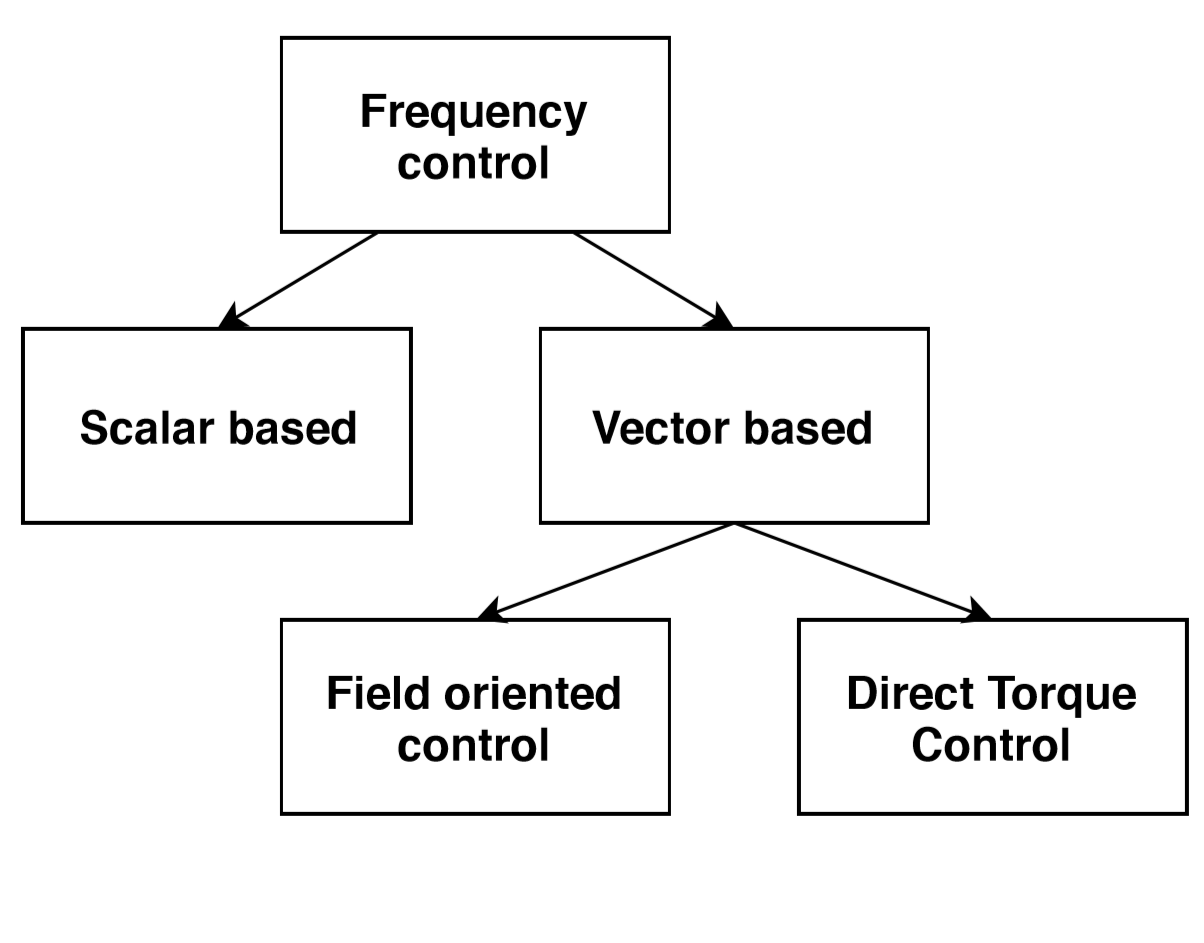
\includegraphics[scale=0.6]{pictures/control/udklip1.PNG}
    \caption{An overview of where FOC is lays among frequency control}
    \label{fig:my_label}
\end{figure} 

The reason for using FOC in this given project, is because it is relatively easy to use and implement. This method gives the control over the current and voltages, and gives information about the orientation of the rotor, which is needed in order to drive the motor forward. \\

It was previously stated that one of the inputs to the motor model was $0$, and it was because of the FOC control. Now the way it controls the rotor, is by having the stator rotational field lead with an 90\textdegree\ electrical degree and having locked there. This is done that maximum torque is gain at this specific angle. So when the Clarke and Park transformation is done, and with the knowledge that the rotor field 90\textdegree\ lacking, after the transformation the rotor and stator becomes parallel and if a rotor- and stator field is no current is running.